% --------------------- VARIABLEN -------------------------

\newcommand{\COURSE}{Physik und Materialwissenschaften\\ Praktikum Physik \\}
\newcommand{\SEMESTER}{Elektro- und Informationstechnik II}
\newcommand{\STUDENT}{Maximilian Spahn\\ und\\Benjamin Langer}

\newcommand{\HEADDING}{Praktikum Physik}
\newcommand{\SUBHEADDING}{Versuch 5.1: Geometrische Optik}

% ------------------- DEFINITIONEN -----------------------

\documentclass[a4paper]{scrartcl}

\usepackage[utf8]{inputenc}
\usepackage[ngerman]{babel}
\usepackage{amsmath}
\usepackage{amssymb}
\usepackage{color}
\usepackage{tikz}
\usepackage{float}
\usetikzlibrary{arrows,decorations.markings}
\usepackage{tabularx}
\usepackage{fancybox}
\usepackage{pgfplots}
\usepackage[colorlinks=false,linkcolor=black,urlcolor=blue,bookmarks,bookmarksopen=true]{hyperref}
\usepackage{geometry}
\usepackage{fancyhdr}

\usepackage[page]{totalcount}

%Größe der Ränder setzen
\geometry{a4paper,left=2cm, right=2cm, top=3cm, bottom=2cm, headheight=8cm}

%Kopf- und Fußzeile
\pagestyle {fancy}
\fancyhf{}
\fancyhead[L]{\STUDENT}
\fancyhead[C]{\COURSE}
\fancyhead[R]{\today}

\fancyfoot[L]{\SEMESTER}
\fancyfoot[C]{}
\fancyfoot[R]{Seite \thepage /\pageref{LastPage}}

%Formatierung der Überschrift, hier nichts ändern
\def\header#1#2{
  \begin{center}
    {\Large #1}\\
    {#2}
  \end{center}
}

\numberwithin{equation}{subsection}

\nocite{*}
\bibliographystyle{plainurl}

\setlength\parindent{0pt}

% ----------------------- DOCUMENT ---------------------------

\begin{document}

\vspace{10pt}
\header{\HEADDING}{\SUBHEADDING}

\tableofcontents

\newpage

\section{Einleitung}

In den folgenden Versuchen werden die verschieden Größen von Linsen und deren optisches Verhalten beobachtet. Dabei wird zunächst im Theorieteil die Lichtbrechung und später das geometrische Verhalten von Linsen erläutert.
Die drei Versuche zeigen weiter die geometrischen Zusammenhänge, zwischen der Brennweite der Linsen und den Abständen von Objekten, sowie deren Bilder, zu der Linse. 
Ebenfalls wird das Besselverfahren zur Bestimmung von Brennweiten beschrieben und angewendet.

\newpage
\section{Theorie}

\subsection{Lichtausbreitung} 

Licht ist eine elektromagnetische Welle. Dabei hält sich das für den Menschen sichtbare Licht zwischen einer Wellenlänge von $780 \;nm$ und $380 \;nm$ \cite{hering}\\

\begin{figure}[H]
\includegraphics[width=12cm]{Abbildungen/Sichtbare-Wellenlaengen}
\centering
\caption{Spektrum des sichtbaren Lichtes \protect\footnotemark}
\centering
\label{fig:sichtbares-licht}
\end{figure}

\footnotetext{\url{https://www.leifiphysik.de/optik/elektromagnetisches-spektrum/grundwissen/sichtbares-licht}}

Die Ausbreitung erfolgt nach Gesetzen einer Welle. Vereinfacht reicht es hier allerdings aus, Licht als einfache Lichtstrahlen zu betrachten. Licht breitet sich mit der Lichtgeschwindigkeit aus, welche im Vakuum mit $c = 299.792.458 \;\frac{m}{s}$.Die Ausbreitungsgeschwindigkeit von Licht in einem Medium $c_n$ ist abhängig vom Medium. In einem dichteren Medium als Vakuum ist die Ausbreitungsgeschwindigkeit geringer. \cite{phys} \\

Beim Übergang des Lichts von einem, zu einem anderen Medium, kommt es durch die unterschiedlichen Ausbreitungsgeschwindigkeiten an der Grenzfläche zu den Phänomenen Reflexion und Brechung. \\

Die Brechzahl $n$ , welche das Verhältnis zu der Lichtgeschwindigkeit im Vakuum beschreibt, wird folgendermaßen definiert\cite{phys}:

\begin{align}
n = \frac{c}{c_n}
\end{align}

Typische Werte für die Brechzahl wären $1,0003$ für Luft und $1,5$ bis $1,66$ für Gläser. \cite{phys}

\subsection{Reflexion und Brechung}
\subsubsection{Reflexion}

Bei der Reflexion werden die einfallenden Wellen von den Atomen der Grenzfläche absorbiert und wieder abgestrahlt

Die abgestrahlten Wellen interferieren nur in einem bestimmten Winkel konstruktiv miteinander. Dieser Winkel ist erreicht, wenn der Einfallswinkel gleich dem Ausfallswinkel.

\begin{figure}[H]
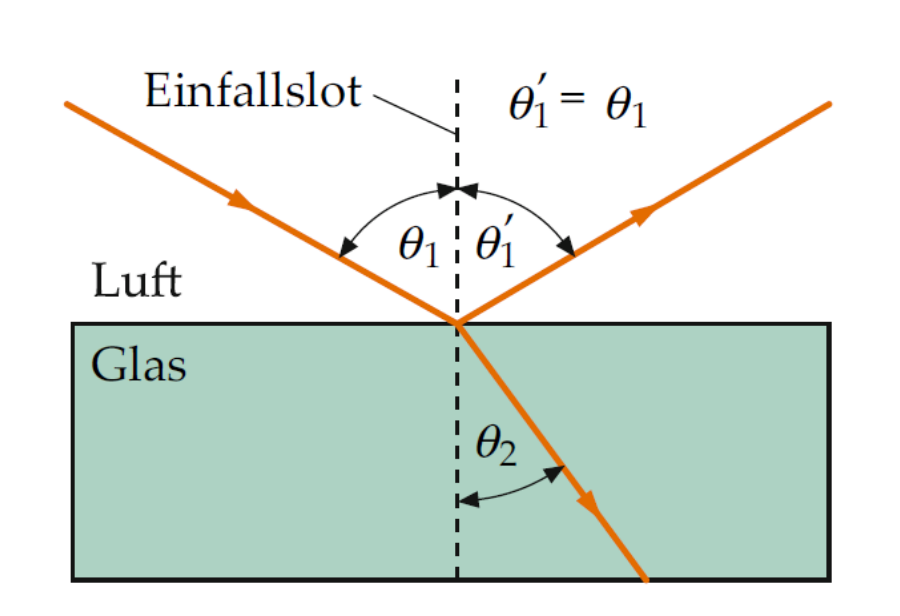
\includegraphics[width=12cm]{Abbildungen/reflexion_und_brechung}
\centering
\caption{Geometrische zusammenhänge von Reflexion und Brechung \cite{phys}}
\centering
\label{fig:reflexion_und_brechung}
\end{figure}

\subsubsection{Brechung}

Wenn parallele Wellenfronten in einem Winkel auf eine Oberfläche treffen, entstehen an den Schnittpunkten der ebenen Wellenflächen mit der Grenzfläche, Huygensscher Elementarwellen. Deren Wellenfronten ergeben entsperchend eines Interferenzmusters neue parallele Wellenfronten und damit die neue Laufrichtung. \cite{phys}

\begin{figure}[H]
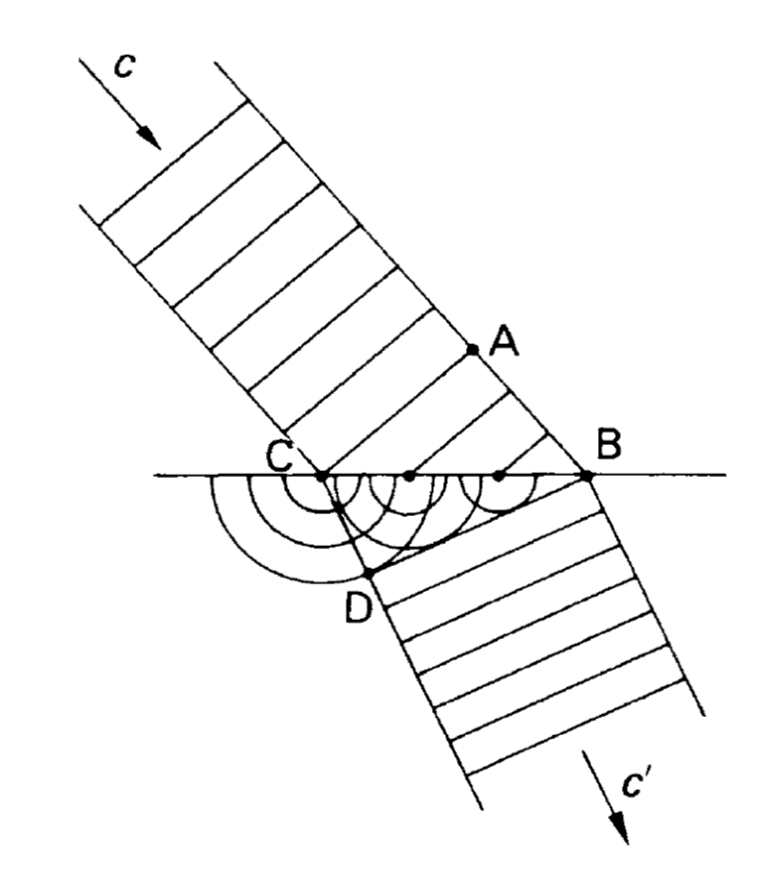
\includegraphics[width=12cm]{Abbildungen/mechanismus-der-brechung}
\centering
\caption{Mechanismus der Brechung \cite{phys}}
\centering
\label{fig:mechanismus-der-brechung}
\end{figure}

Der Winkel der neuen Wellenfront ergibt sich nach dem Senelliusschen Brechungsgesetz: \cite{hering}

\begin{align}
n_1 \cdot \sin(\theta_1) = n_2 \cdot \sin(\theta_2)
\end{align}


\subsection{Linsen}
Linsen sind eines der wichtigsten optischen Instrumente. Bei Linsen wird die Brechung des Lichtes an der Oberfläche, mithilfe einer bestimmten Geometrie, genutzt, um Licht entweder zu bündeln oder zu streuen.
Das Verhalten der Linse hängt von ihrer Form ab: \cite{anl}

\begin{figure}[H]
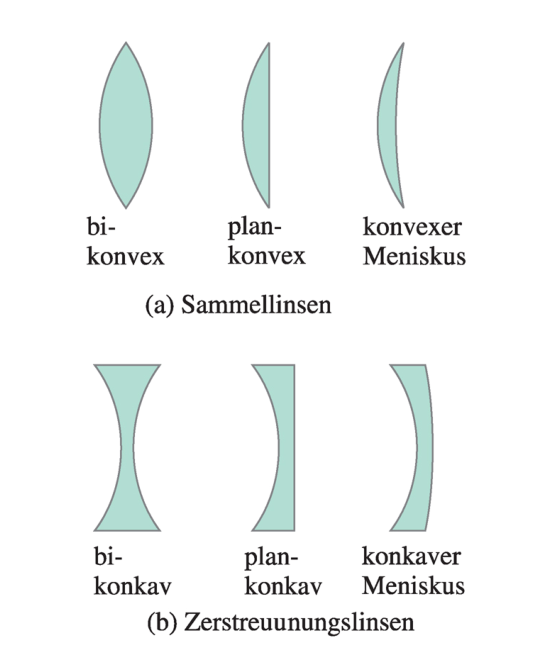
\includegraphics[width=12cm]{Abbildungen/linsentypen}
\centering
\caption{Linsentypen \cite{anl}}
\centering
\label{fig:linsentypen}
\end{figure}

Alle Linsen haben zwei Brennpunkte. Diese Brennweite $f$ einer Linse (also der Punkt in dem das Licht gebündelt wird) lässt sich aus dem Radius ihrer Wölbung und ihrer Brechzahl bestimmen: \cite{anl}

\begin{align}
\frac{1}{f} =  \left( \frac{n}{n_{\textit{Luft}}} - 1 \right) \cdot \left( \frac{1}{r_1} - \frac{1}{r_2} \right)
\end{align}

Der Kehrwert der Brennweite heißt Brechkraft:

\begin{align}
D = \frac{1}{f} \qquad [D] = 1 \;dpt \; \text{Dioptrie}
\end{align}

\subsection{Geometrische Optik}

Linsen können genutzt werden, um eine Abbildung eines Objektes zu erzeugen. Um deren Verhalten geometrisch zu beschrieben, wird ein Strahlendiagramm benutzt. Dafür zeichnet man drei spezielle Strahlen ein: den Mittelpunktstrahl, den Parallelstrahl und den Brennpunktstrahl. Alle drei Strahlen gehen auf der Gegenstandsseite durch die Spitze des Objekts.\\

Im Weiteren werden hier nur die Sammellinsen (oder auch bi-konvexen Linsen) betrachtet. \cite{anl}
Für diese gilt:\\
• Der Mittelpunktstrahl geht durch den Mittelpunkt der Linse und wird nicht gebrochen. \\
• Der Parallelstrahl fällt parallel zur optischen Achse ein und wird so zur Achse gebrochen, dass er durch den hinteren Brennpunkt geht. \\
• Der Brennpunktstrahl geht durch den vorderen Brennpunkt und wird so zur Achse gebrochen, dass er hinter der Linse parallel zur optischen Achse verläuft. \\

Der Punkt in dem sich die abbildenden Strahlen treffen, ist der Punkt in dem die Abbildung entsteht.\\

\begin{figure}[H]
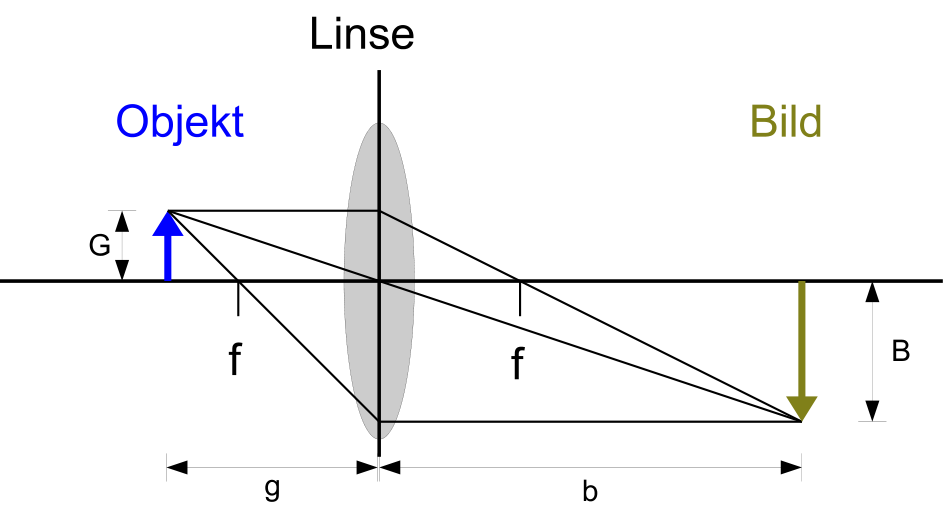
\includegraphics[width=12cm]{Abbildungen/strahlendiagramm}
\centering
\caption{Strahlendiagramm \cite{anl}}
\centering
\label{fig:strahlendiagramm}
\end{figure}

Wenn ein Objekt weiter entfernt ist als die Brennweite der Linse, entsteht auf diese Weise eine reale Abbildung auf der entgegengesetzten Seite der Linse. Die Linse arbeitet in diesem Fall als Linse. Wenn das Objekt jedoch näher ist als die Brennweite der Linse, treffen sich die reellen Stahlen nicht auf der anderen Seite der Linse. In diesem Fall liegt eine virtuelle Abbildung vor und die Linse arbeitet als Lupe. Diese virtuelle Abbildung entsteht wo sich die geradlinigen Rückverlängerungen der abbildenden Lichtstrahlen schneienden.\\

\begin{figure}[H]
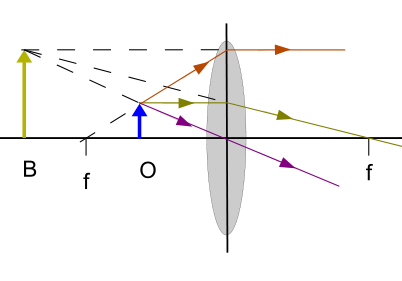
\includegraphics[width=12cm]{Abbildungen/strahlendiagramm2}
\centering
\caption{Strahlendiagramm virtuelles Bild\cite{anl}}
\centering
\label{fig:strahlendiagramm2}
\end{figure}

Mathematisch lässt sich das Verhalten der Linsen durch die Gleichung

\begin{align}
\frac{1}{f} = \frac{1}{g} + \frac{1}{b}
\end{align}

beschreiben.\cite{anl} \\
Dabei ist $f$ die Brennweite der Linse, $g$ ist der Abstand des abzubildenden Objektes zu der Linse und $b$ der Abstand der Abbildung zu der Linse.
Für den Fall das eine virtuelle Abbildung vorliegt, lässt sich mit der Gleichung ein negativer Wert für $b$ berechnen. Dementsprechend liegt das virtuelle Bild auf derselben Seite wie das abgebildete Objekt.\\

Durch das Verwenden einer zweiten Linse kann dieses virtuelle Bild genutzt werden, um ein vergrößertes oder verkleinertes reelles Abbild zu erzeugen. (Für die Anwendung dieser Funktionsweise, siehe häusliche Vorarbeit)

\subsubsection{Abbildungsmaßstab}

Der Abbildungsmaßstab eines optischen Instruments ist definiert als das Verhältnis von Bildgröße zu Gegenstandsgröße. Für eine dünne Linse gilt: \cite{anl}

\begin{align}
\frac{B}{G} = \frac{\vert b \vert}{g}
\end{align}

\subsection{Das Bessel-Verfahren}

Eine Methode die Brennweite einer Linse zu messen ist das Verfahren nach Bessel. Dabei wird eine Gegenstand in einem Abstand $s$ zum Schirm platziert. Der Abstand sollte dabei größer sein als vier Mal die Brennweite. Wird nun eine Linse mit unbekannter Brennweite dazwischen platziert, gibt es zwei Positionen, in welchen eine scharfe Abbildung entsteht.
Der Abstand zwischen den beiden Linsenpositionen $e$ und der Abstand zwischen Objekt und Schirm $s$ genügt um die Brennweite zu bestimmen. \cite{anl}

\begin{figure}[H]
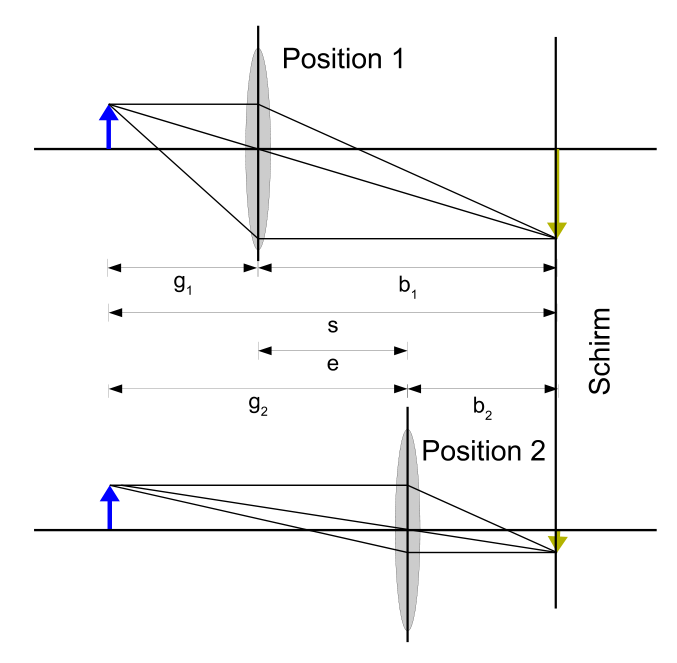
\includegraphics[width=12cm]{Abbildungen/bessel_brennweitenbestimmung}
\centering
\caption{Brennweitenbestimmung nach Bessel\cite{anl}}
\centering
\label{fig:bessel_brennweitenbestimmung}
\end{figure}

\begin{align}
f = \frac{1}{4} \cdot \left( s - \frac{e^2}{s} \right)
\end{align}

Zur Messung der Brennweite werden die relativ schwer zu messenden Größen $g$ und $b$ nicht mehr benötigt, was die Messung einfacher und genauer macht.

\newpage
\section{Häusliche Vorarbeit}

\subsubsection{1:1 Abbildung}

Da $B = G$ sein soll (1:1 Abbildung) muss nach:

\begin{align*}
\frac{B}{G} = \frac{\vert b \vert}{g}
\end{align*}

auch $b=g$ sein.\\

Aus der Linsengleichung nach $b$ bzw. $g$ umgestellt ergibt sich:

\begin{align*}
\frac{1}{f} = \frac{1}{g} + \frac{1}{b} \quad \Rightarrow \quad \frac{1}{f} &= \frac{1}{g} + \frac{1}{g} \\
\frac{1}{f} &= \frac{2}{g} \\
g = b &= 2 \cdot f
\end{align*}

Die Zeichnung zeigt ebenfalls diesen Zusammenhang:

\begin{figure}[H]
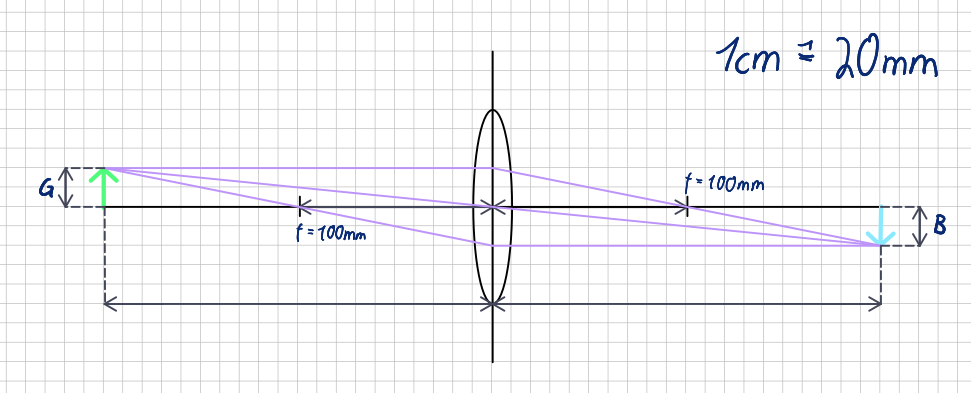
\includegraphics[width=12cm]{Abbildungen/zeichnung_linse}
\centering
\caption{Strahlendiagramm: 1:1 Abbildung}
\centering
\label{fig:zeichnung_linse}
\end{figure}

\subsubsection{1:2 Abbildung}

Um eine vergrößerte, virtuelle Abbildung zu erzeugen, muss sich das Bild innerhalb der Brennweite der Linse befinden.
Damit $B = 2 \cdot G$ ist, muss auch $b = 2 \cdot g$ sein.

\begin{figure}[H]
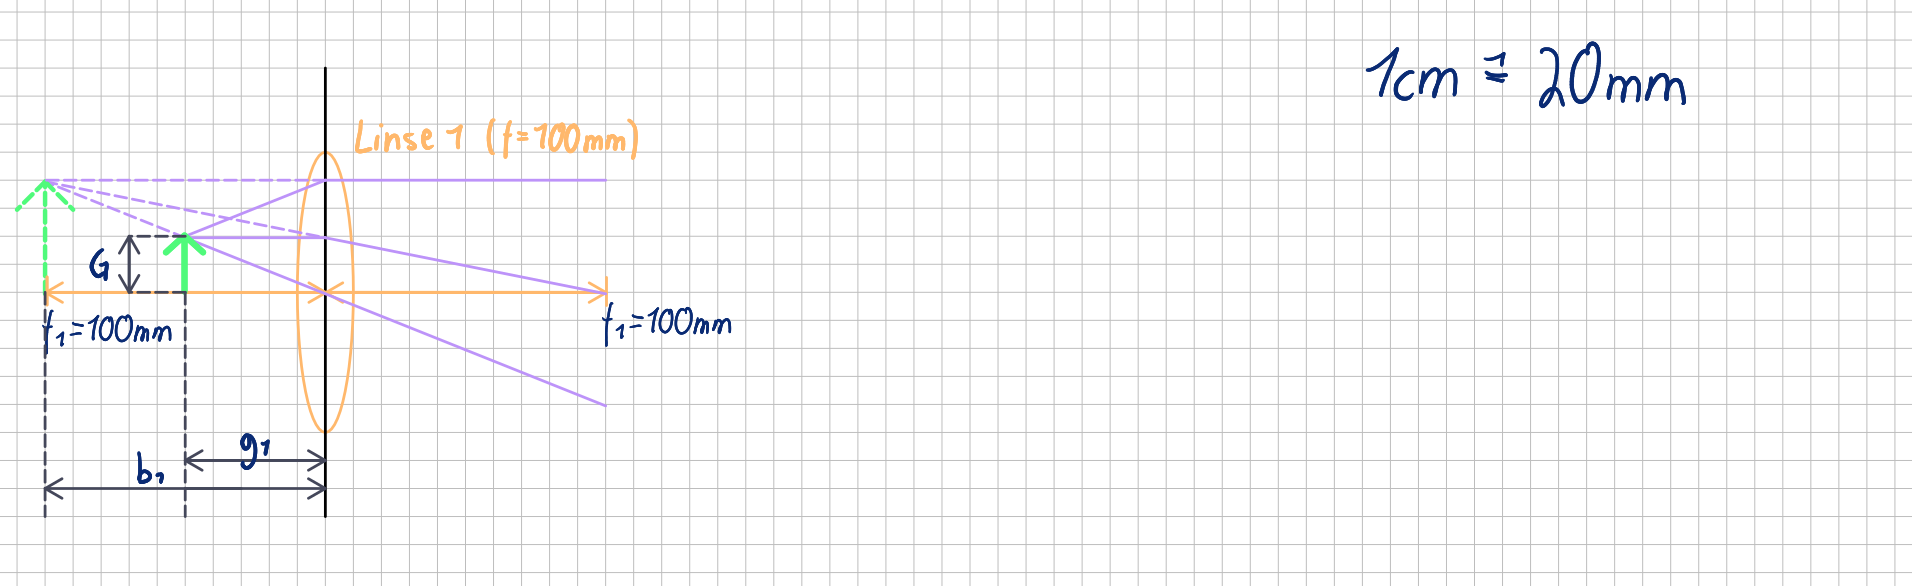
\includegraphics[width=16cm]{Abbildungen/zeichnung_zwei_linsen_1}
\centering
\caption{Strahlendiagramm: 1:2 Abbildung (Teil 1)(größer im Anhang)}
\centering
\label{fig:zeichnung_zwei_linsen_1}
\end{figure}

Um von dem virtuellen Bild eine reelle Abbildung zu erzeugen wird eine zweite Linse benötigt. Da diese eine 1:1 Abbildung erzeugen soll, muss diese mit der bereits oben hergeleiteten Bedingung platziert werden:

\begin{align*}
g = b &= 2 \cdot f
\end{align*}

Der erweiterte Aufbau sieht wie folgt aus:

\begin{figure}[H]
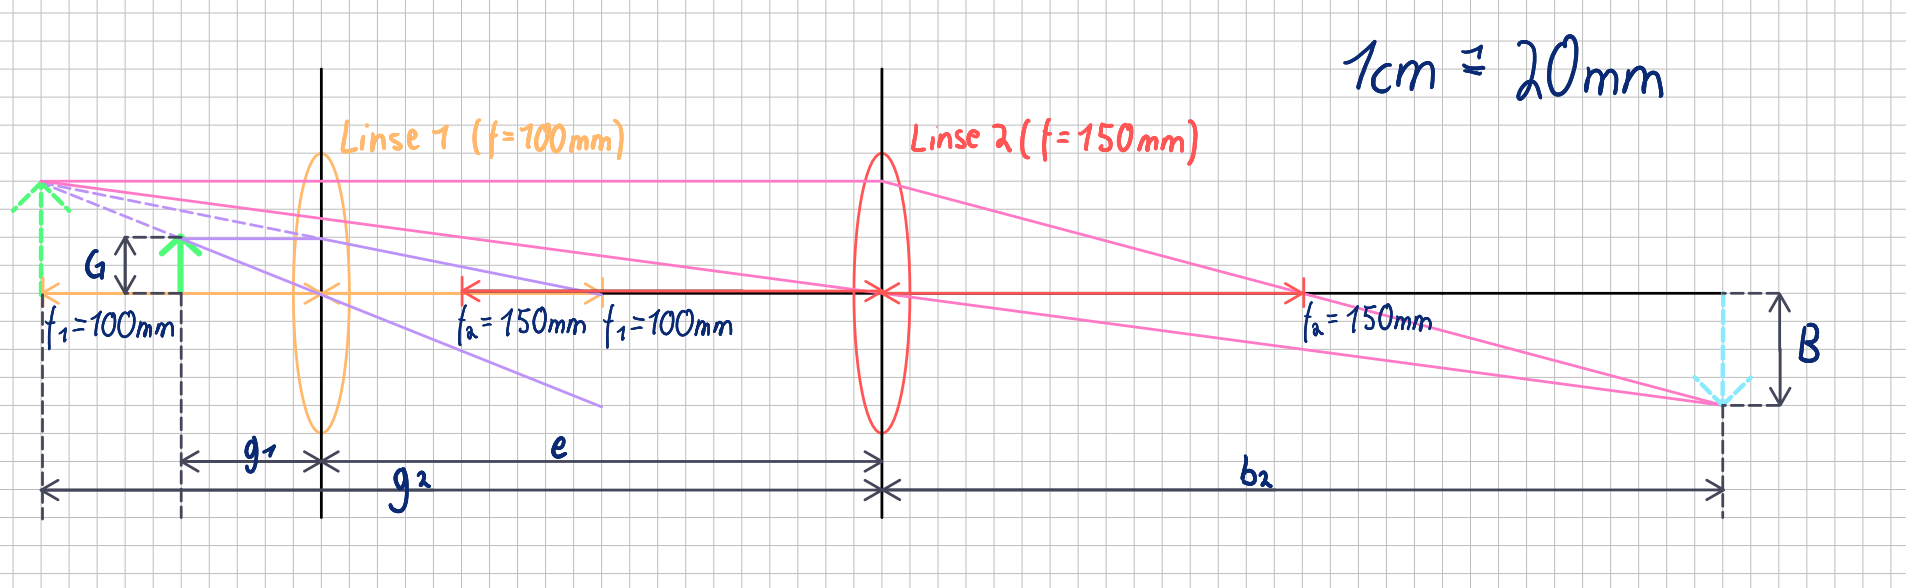
\includegraphics[width=16cm]{Abbildungen/zeichnung_zwei_linsen_2}
\centering
\caption{Strahlendiagramm: 1:2 Abbildung (Teil 2)(größer im Anhang)}
\centering
\label{fig:zeichnung_zwei_linsen_2}
\end{figure}

\newpage
\section{Aufbau und Durchführung}

Der Aufbau besteht aus einer Lampe und einem Dia mit einem Pfeil, der als Objekt dient, einem Schirm sowie verschiedene Linsen, die auf einer optischen Bank montiert werden können.

\begin{figure}[H]
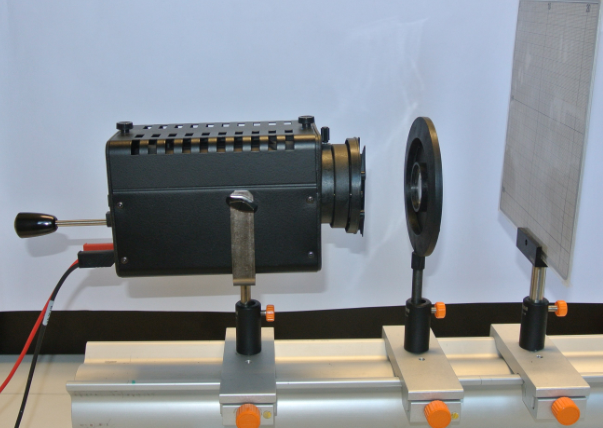
\includegraphics[width=8cm]{Abbildungen/versuchsaufbau}
\centering
\caption{Versuchsaufbau \cite{anl}}
\centering
\label{fig:versuchsaufbau}
\end{figure}

\subsubsection{Teil A: 1:1 Abbildung}

Mithilfe einer Konvex-Linse soll eine 1:1 Abbildung des Dias erzeugt werden. Dazu wird die Linse auf der optischen Bank befestigt und die Abstände von Linse und Schirm entsprechend angepasst. 

\subsubsection{Teil B: Bessel}

Für die Linse aus Teil A wird nun die Brennweite bestimmt. Dazu wird das Bessel-Verfahren, wie es im Theorieteil beschrieben wurde, angewendet. Dabei werden Dia und Schirm mit einem Abstand, größer als 4-mal die angenommene Brennweite der Linse platziert und dieser Abstand gemessen. Anschließend werden die zwei Positionen gesucht, in welchen die Linse ein scharfes Bild liefert. Der Abstand zwischen den beiden Positionen wird ebenfalls gemessen.

\subsubsection{Teil C: Lupe}

Zunächst wird eine Konvex-Linse $L_1$ so befestigt, dass diese als Lupe mit einer 1:2 Vergrößerung wirkt. Anschließend wird eine zweite Konvex-Linse so angeordnet, dass das vergrößerte, virtuelle Bild 1:1 auf den Schirm abgebildet wird.

\newpage
\section{Auswertung Versuch}

\subsubsection{Teil A: 1:1 Abbildung}

Bei der genutzten Linse konnte mit den Abständen $g = (199 \mp 4) \;mm$ und $b = (198 \mp 4) \;mm$ ein scharfes Bild erzeugt werden.
Die Größe des Dias betrug $B = (10 \mp 1) \;mm$ und die Größe der Abbildung war $B = (10 \mp 1) \;mm$. Somit lag eine näherungsweise 1:1 Abbildung vor. 
Aus den gemessenen Größen lässt sich die Brennweite berechnen:

\begin{align}
\frac{1}{f} &= \frac{1}{g} + \frac{1}{b} \\
f_{\textit{exp.}} &= \frac{1}{\frac{1}{g} + \frac{1}{b}} \\
					&= 96,935 \;mm
\end{align}

\textit{Fehlerrechnung:}

\begin{align*}
\frac{\partial}{\partial b} f_{\textit{exp.}} &= 	\dfrac{g^2}{\left(b+g\right)^2}	 \\
\frac{\partial}{\partial g} f_{\textit{exp.}} &= \dfrac{b^2}{\left(g+b\right)^2}
\end{align*}

\begin{align*}
U_{f_{\textit{exp.}}} = \bigg | \frac{\partial}{\partial b} f_{\textit{exp.}} \bigg | \cdot U_{b} + 
					    \bigg | \frac{\partial}{\partial g} f_{\textit{exp.}} \bigg | \cdot U_{g} = 2,100 \;mm
\end{align*}

\begin{align*}
f_{\textit{exp.}} = (96,9 \mp 2,1) \;mm
\end{align*}

Verglichen mit dem tatsächlich auf der Linse angegeben Wert von $f = 100 \;mm$ verglichen ist das gemessene Ergebnis sehr in der Nähe, aber nicht wirklich genau.
Die beobachtete Messunsicherheit entsteht vor allem dadurch, dass sich die genaue Mitte der Linse nicht genau messen lässt, da diese von der Befestigung/Rahmen verdeckt ist.


\subsubsection{Teil B: Bessel}

Durch Verwendung des Bessel-Verfahrens wurden folgende Werte gemessen:

\begin{align*}
e =& (155 \mp 1) \;mm \\
s =& (451 \mp 2) \;mm
\end{align*}

Daraus lässt sich die Brennweite berechnen:

\begin{align}
f_{\textit{bessel}} = \frac{1}{4} \cdot \left( s - \frac{e^2}{s} \right) = 99,4323 \;mm
\end{align}

\textit{Fehlerrechnung:}

\begin{align*}
\frac{\partial}{\partial e} f_{\textit{bessel}} &= \dfrac{e}{2s}		 \\
\frac{\partial}{\partial s} f_{\textit{bessel}} &= \dfrac{\frac{e^2}{s^2}+1}{4}
\end{align*}

\begin{align*}
U_{f_{\textit{bessel}}} = \bigg | \frac{\partial}{\partial e} f_{\textit{bessel}} \bigg | \cdot U_{e} + 
					    \bigg | \frac{\partial}{\partial s} f_{\textit{bessel}} \bigg | \cdot U_{s} = 0,731
\end{align*}

\begin{align*}
f_{\textit{bessel}} = (99,43 \mp 0,74) \;mm
\end{align*}

Verglichen mit dem in A bestimmten Wert ist das über das Bessel-Verfahren bestimme Ergebnis deutlich genauer und entspricht auch mehr dem tatsächlichen Wert der Linse. \\

Die Messunsicherheiten sind hier deutlich geringer, da sich $e$ und $s$ deutlich leichter messen lassen. Dies liegt daran, dass für $e$ nicht die genaue Mitte der Linse bestimmt werden muss, sondern nur ein fixer Punkt an der Befestigung genutzt werden kann, um den Abstand zwischen den beiden Positionen zu bestimmen.


\subsubsection{Teil C: Lupe}

Nach den, in der häuslichen Vorarbeit hergeleiteten Zeichnungen (Abbildung [\ref{fig:zeichnung_zwei_linsen_2}]) und Gleichugen, lassen sich die Linsenabstände wie folgt brechen.
Im folgenden wird für die erste Linse, eine Linse mit einer Brennweite von $f = 100 \;mm$ genutzt, als zweite Linse wird eine Linse mit $f = 150 \;mm$ genutzt:
Für die Position der ersten Linse gilt:

\begin{align*}
b = 2 \cdot g \quad \text{und} \quad \frac{1}{f} = \frac{1}{g} + \frac{1}{-b}
\end{align*}

\begin{align*}
\textit{(b muss negativ sein, da es ein virtuelles Bild ist)}
\end{align*}

\begin{align*}
\frac{1}{f} &= \frac{1}{g} - \frac{1}{2g} \\
\frac{1}{f} &= \frac{1}{2g} \\
f &= \frac{2}{1}\cdot g \\
g &= \frac{1}{2}\cdot f
\end{align*}

Daraus ergibt sich für $g_1$ und $b_2$:

\begin{align*}
	g_1 &= 50 \;mm\\
	b_1 &= 100 \;mm
\end{align*}

Für die Position der zweiten Linse gilt:

\begin{align*}
b = g \quad \text{und} \quad g = b &= 2 \cdot f
\end{align*}

Daraus ergibt sich für $g_2$ und $b_2$:

\begin{align*}
	g_2 &= 300 \;mm\\
	b_2 &= 300 \;mm
\end{align*}

In der Realität kann $g_2$ nicht wirklich gemessen werden.
Dafür kann $e$ ermittelt werden und daraus $g_2$ berechnet werden. \\

Als optimierte Abstände wurden somit

\begin{align*}
	G &= (10 \mp 1) \;mm\\
	B &= (19 \mp 1) \;mm\\
	g_1 &= (52 \mp 2) \;mm\\
	b_1 &= (105 \mp 2) \;mm\\
	g_2 &= (301 \mp 2) \;mm\\
	b_2 &= (300 \mp 2) \;mm
\end{align*}

gemessen.\\

Diese Werte liegen wie erwartet sehr nahe, bei den bereits errechneten Werten.

\newpage
\section{Wertung/Fazit}

Auch wenn das Messen der Werte für $g$ und $b$ nicht ganz einfach und genau ist, konnten dennoch die berechneten Werte in den einzelnen Versuchs-Teilen gut bestätigt werden. Wie diese Ungenauigkeit zu stande kommt wurde bereits an entsprechender Stelle erläutert. Die Bessel Methode ist jedoch ein guter Weg, die Messungenauigkeiten von $g$ und $b$ zu umgehen. Wie auch an den Messergebnissen zu sehen war, konnten so deutlich genauere Werte ermittelt werden.

\newpage
\section{Anhang}

\begin{figure}[H]
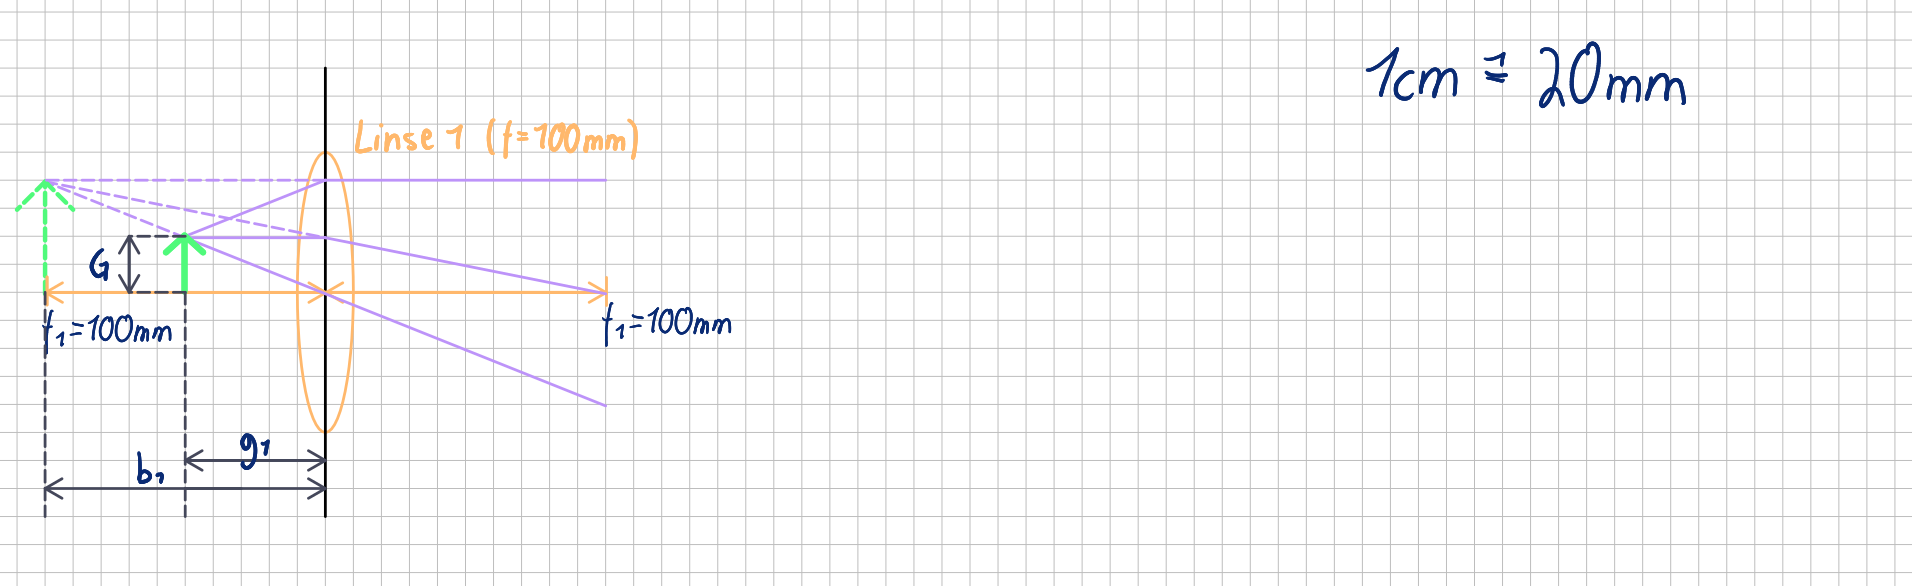
\includegraphics[width=20cm, angle=90]{Abbildungen/zeichnung_zwei_linsen_1}
\centering
\caption{Strahlendiagramm: 1:2 Abbildung (Teil 1)}
\centering
\label{fig:zeichnung_zwei_linsen_1}
\end{figure}

\begin{figure}[H]
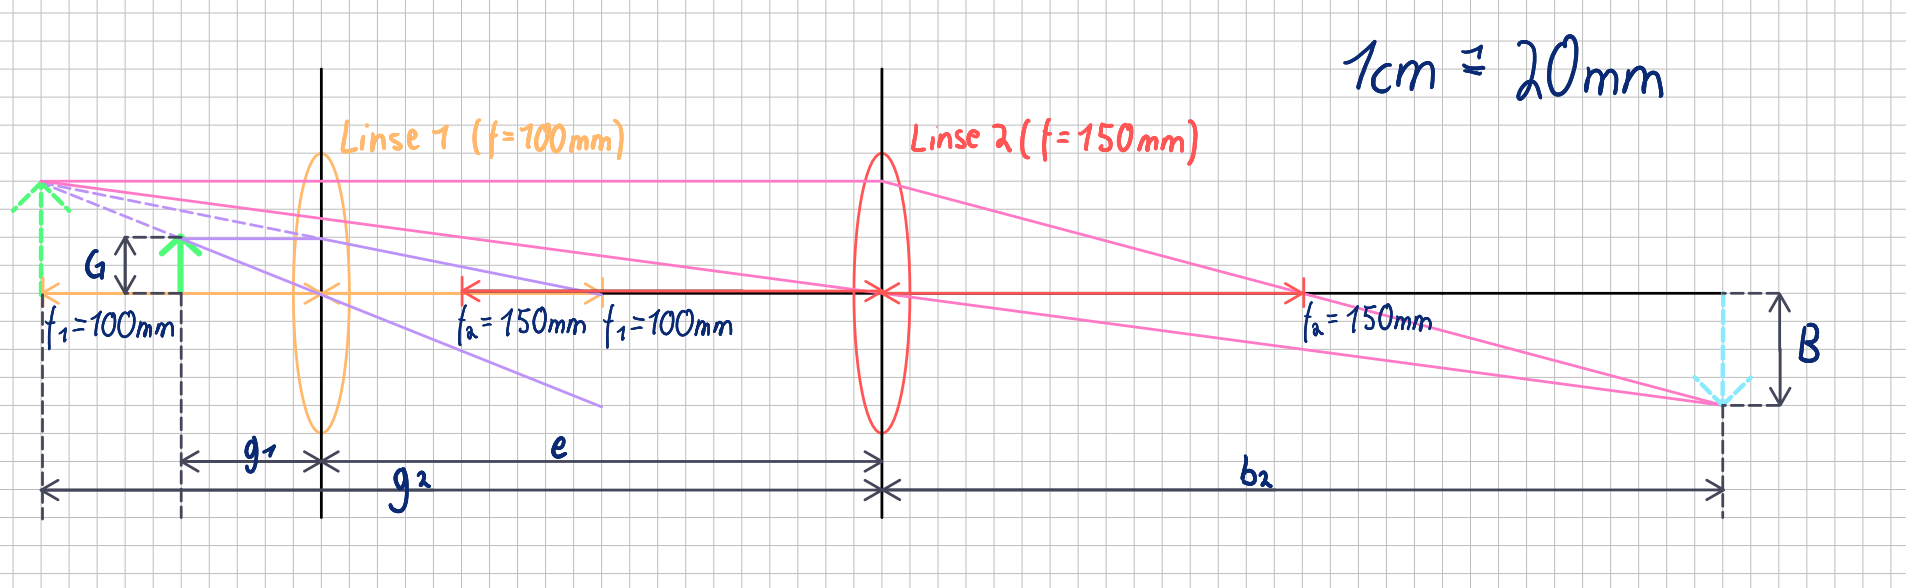
\includegraphics[width=20cm, angle=90]{Abbildungen/zeichnung_zwei_linsen_2}
\centering
\caption{Strahlendiagramm: 1:2 Abbildung (Teil 2)}
\centering
\label{fig:zeichnung_zwei_linsen_2}
\end{figure}

\newpage
\bibliography{literatur}

\label{LastPage}

\end{document}
%%% Local Variables:
%%% mode: latex
%%% TeX-master: t
%%% End:
